\documentclass[ebook,12pt,openany]{memoir} %ebook

%\documentclass[ebook,12pt,openany,onesided]{memoir} %physical book

\usepackage[utf8x]{inputenc}
\usepackage[english]{babel}
\usepackage{url}
\usepackage{graphicx}
\usepackage{imakeidx} % for how to use the index see https://www.sharelatex.com/learn/Indices
\usepackage{hyperref}

\makeindex


\title{The Organic Web \\ Social media of replication}
\author{Lafe Spietz}

\begin{document}
\frontmatter
\begin{figure}[htbp]
\centering
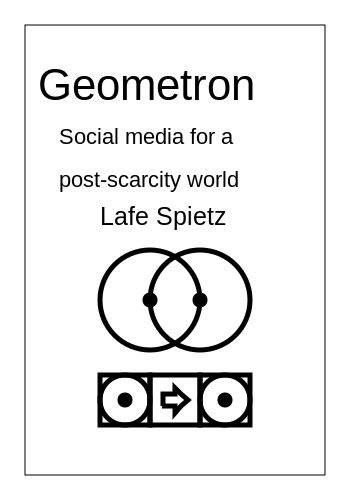
\includegraphics{cover.png}
\end{figure}

\clearpage

\clearpage

\newpage
\thispagestyle{empty}
\mbox{}

\maketitle

\tableofcontents

\listoffigures 

%civilizations
%

\mainmatter

\chapter{Civilizations}


\subsection{Consumer Civilization}

The nature of our present civilization is one of constant consumption.
We mine or drill material out of the ground, re-shape it or burn it for
fuel, and ultimately turn it into toxic waste which we dump back into
the environment. During the process from mine to landfill, we exchange
``money'' and this is what we call the ``economy''. The things which can
be exchanged for money are called ``property''.

Mining.  Each mineral is absolutely needed by whole system. Each is critical.  Rare earths.  Exotic transition metals. Lithium batteries.  foreshadowing of where all this is going by closing the loops, examples. 

Centralized mass production.  The fab.  

Globalized consumer supply web.

Universal replication of structure of waste stream.

The purpose of media in consumer civilization: to stimulate consumption.  Not just through advertising but through legitimizing the power structures required to maintain consumption, both corporate power and the power of the state.

\subsection{Organic Civilizations}

In mature civilizations, technology is all self-replicating. We look to the technological civilizations of
indigenous people as an example of what mature technology should look
like. These civilizations are based not on a stream from
mine to landfill, but on closed loops of material in equilibrium with
living ecosystems. 


An example of technology in a mature civilization is traditional wooden
boats. If people live in equilibrium with a forest, as old trees die or
are harvested new trees grow. People carve logs into boats, and then use
them to hunt and sustain their communities. A new generation of humans
is born from the old, and they are taught all the skills to copy the
construction of the boat, the stewardship and harvesting of the trees,
and how to pass along the knowledge of boat building(as well as the
hunting and fishing that sustains the whole society) to the next
generation after them and so on. Unlike a consumer civilization, this
type of self-replicating organic technology can continue in theory
indefinitely. If it has the resilience built in to improve and change
over time in response to changes in the ecosystem it can truly sustain
itself without limits. Mature civilizations like this have existed for
thousands of years all over the Earth.

Three things to note about a technology such as the one described above:
everything replicates, everything can be modified, and everything dies.
Every wood boat will rot, and eventually become soil again in the forest
which will produce more trees. The technology is soft enough that people
can modify it, carve and repair it over time, change it as needed, and
evolve it as needed in response to changing conditions in the
environment or new innovations in the technology. And of course, every
boat can always be copied freely. In this context the idea of property
doesn't make sense. Nothing is permanent. Everything is constantly going
through a cycle from soil to tree to boat to soil again, growing,
evolving dying, and being reborn.


\subsection{What comes next? Opportunities!}


The false dichotomy of ``progress''.  There will never be another stone age.

The structure of the trash feed.

A picture of what civ could look like based on trash feed.

\subsection{Goals and Methods}

is this its own section? do we just cut all this and have previous section point to organic media as the path forward?

So what is the alternative? The alternative is a switch from an
arithmetic to a geometric economy. This means that rather than an
economy of exchange, where numbers are used to represent both property
and labor, we have an economy of replication of geometric constructions.
In this situation, the replication of information \emph{is} the economy.
It does not turn into numbers at any point. One can create a thing via a
geometric construction from trash which contains information for its own
replication. This then replicates out into the human network in a
replication-based future descendant of the current Internet, and we all
share the increased value. When we create value we do not ``trade'' it
for something, because the amount of value will \emph{increase} as it
replicates, making any trade that truly represents the added value
impossible. In a post-scarcity trash-sourced geometric economy, everyone
benefits from the creation of creators because the best things naturally
replicate to all of humanity, including the back to the creators
themselves, but now amplified by the added benefit of billions of people
potentially improving it.

The Geometron/Trash Robot system is an attempt to build an information
technology system which serves this purpose: to build a purely geometric
economy based on replication. In this system, everything replicates,
everything evolves, and everything can be deleted at any time. In the
beginning we source some parts from trash and some parts from common off
the shelf consumer items that are easy to buy without any centralized
company. In order to replicate successfully, however, this information
networking system has to provide immediate value to the user, both
within the existing money-based economy, and also outside that system.

In order for all this to work, we have to give up the three main
elements of our existing system: mining, money, and property. As long as
money exists, replication will break the economy. As long as mining
exists, we will continue on a path to total destruction of the world and
eventually scarcity and extinction. And as long as property exists,
replication which could end all scarcity for all of humanity will be
hindered by the people who control everything. The extension of property
into the domain of pure information is another major reason that people
in the replication industries have been able to so brutally exploit the
rest of humanity. They claim to ``own'' most of the freely replicating
information we rely on in the new economy, and they're effectively
landlords who can create new land as many times as they want for free,
but then can charge rent on all of it. Only by creating a new economic
model from scratch which simultaneously abandons money, mining and
property, can we build a just and sustainable future.

It is not immediately obvious that geometry can completely replace
numbers-based thinking. But in most cases, our technology is already
completely driven by geometry, we just choose not to look at it that
way. What is a microchip? It is a geometric design imprinted in silicon.
That design is made by a geometric program interacted with by a user
thinking geometrically. Even the code itself, encoding into the physical
circuits, is a geometric pattern of either magnetic or electric
perturbations of physical objects. And ``computers'' are not used
primarily to compute things, but to display graphical information, both
text and pictures and graphics. The repeated actions of automation
machinery represent geometric operations(e.e. move over, move up, move
down, move over, etc\ldots{})

Saying ``geometric economy'' sounds abstract and to say it
self-replicates sounds far fetched, but none of this is a new idea. Many
of the oldest and most sustainable civilizations in the world have very
very old technologies involving textiles made from natural materials
woven into patterns. This is self-replicating geometry. It satisfies all
the properties listed here: it dies of natural decay, is taught as a
skill from the old to the young and is constantly replaced, and it can
be modified and improved over time by the constantly-replicating group
of experts in the technology within the community. So the transition to
a geometric economy is not to some futuristic new idea but a return to
ideas which predate the rise of industrial societies and nation-states.

All that said, we live in times different from any which came before.
The Internet is the baseline information system now for all of humanity.
Even the few people not connected to the Internet now have their lives
completely molded by it, as all power networks exist on it now. And
consumer society has injected every single element or type of finished
product our civilization uses all over the planet. So while in times
before now one group of people might discover the use of bronze and
another of steel, now every single person on the planet can get aluminum
sheet metal, titanium reinforced steel, rare earth metals, ultra high
purity silicon, etc. All these incredible materials, already shaped and
processed into the most useful form, are simply sitting in piles of
trash in every corner of every nation on the planet now, all directly
adjacent to nodes on an information network which connects to every
other part of the planet.

This combination of universal networking and universal access to
identical, standardized, trash elements creates a formula for building a
new information system from scratch from which a whole stream of new
civilizations can rise. It is our task to build a seed from which such
civilizations can be built. Geometron is an attempt to build this seed.

This chapter encapsulates the Trash Magic Manifesto and references it.  It sets up the problem at the highest level before delving into the specifics of the solution.  This chapter describes the problem that all subsequent chapters provide the solution for.  Essentially the Trash Magic Manifesto laid out a goal for technology and for civilization.  I realized that information technology has to form the basis of all the other technology.  If information technology is taken to be general enough, it can be the basis of the entire complete set defined in the Trash Magic Manifesto.  Define that set here.  Generalized media. Point to the next chapter.
\chapter{Organic Media}
\url{index.html}

\section{Organic Media}\label{organic-media}

\begin{itemize}
\item
  everything replicates
\item
  everything evolves
\item
  everything dies
\item
  no money
\item
  no mining
\item
  no property
\end{itemize}

Organic media exist to replicate that which we desire to replicate.  Its purpose is to facility replication of things.  It contains both information on how to replicate things and information required to inspire people to \emph{desire} to carry out replication.  We must give people a reason to replicate as well as a means to replicate.  Thus one form of Organic Media is instructions on how to build something you can sell.  To maximize replication we are less concerned with how much money someone can make via replication than we are with how little they have to spend to initiate replication.  We want to minimize the cost of each item a person might buy to sell, the minimum number required to be purchased, and also minimize the amount of labor and skill required to make the thing.  The ArtBox is an example: each box contains the content to make another box.  Each box is awesome and can be sold.  The ArtBox itself is Organic media.  a bunch of SRS gets moved here.



path of replication: how to install and how to teach others to install,
how to replicate the code, replicate specific files, how it's all
structured, editing the code itself

the structure of sign pointing to domain which points to terminal which
is near a place which is labelled by domain(this needs to get explained
early since it will be the referenced in everything, as it's basic to
the structure of the System)

Editing: how files work, how they don't work. No databases. no private
data. No file that cannot be edited.

Deletion: cheap sd cards can be wiped any time. All files can be deleted
or written over by anyone at any time. Domains are chosen to be of no
real value, are disposed of as soon as burned, never sold. Evaluate
entropy of domain names to prove we can always have zero value of names
even as our network grows exponentially. ``Permanent'' deletion less
critical in a world without private or personal data.

Cybersecurity: there is none. Security is for private property, and
there simply is none on this network. This network must always be
disconnected from the property-based Internet or private systems. One
way paths of information for protection.

draw from the SRS paper and the existing organic media paper(but the
formal SRS idea goes in ontology chapter)

File types independent of technology: symbols, feeds, maps, scrolls.
These can be described without any specific implementation of
\emph{either} software \emph{or} hardware. Specific implementations will
be dealt with in their own sections.

How files are structured, overview of file types, what they do. All of
this is as a generalized specification which users can use to rewrite
from scratch quickly.

Example of physical organic media: The Art Box, replicator card,
replicator shape, object itself, scroll

We will return to the Art Box again and again as we go through the
system, illustrating how it can replicate in the Geometron system and
how it fits into all the parts: symbols in ``symbols'' for the shapes
and net, the set in ontology, maps, feeds, scrolls, scroll replicator,
role in magic as one of the Trash Robot avatar objects

The user page, basic operation of Geometron as it exists today, just
viewing now editing, but with pointers to editors, jump on and look at a
file RIGHT NOW, on one of my pages.

In organic media chapter we introduce geometron and say what we're going
to be doing in this book. What we are doing is providing a
\emph{specification} and an \emph{example} of an instance of that spec.
We will use the Pi, and remote hosted pages. But expect this spec to be
used by many coders on many platforms in many ways if successful.

\chapter{Street Network}

\section{Street Network}



outline:
\begin{itemize}
  \item
  what and Why?  The power of the physical, local, and free.  Organic media, what we want, links to previous chapter.  Universal social media for sharing of information in a physically local domain with both content creation and consumption on all Web-enabled devices(laptops, phones, tablets, etc.)  Hybrid markets: like Craigslist, but way more local.  General description of what the system does(scrolls,maps, feeds, symbols, apps, industrial design and production via Trash Robot). This points to the subsequent chapters about these actual things.  Free boxes and food not bombs.  We are a hybrid between free boxes and food not bombs and craigslist.
  \item
  The Terminal.  This is the heart of this system. What is the Raspberry Pi, why is it powerful?  How to build the Terminal. Options involving big screens and projectors, public terminals with large publicly viewable displays.  How to adapt it to different situations, how to work with wifi networks, IP addresses, local and global, opening up a local wifi to a public domain.  how to avoid ANY property.  How the terminal is passed from user to user to operator to operator.  Data hygiene: how to keep all personal information of any kind of the machine, to prevent leaks of property.  What it means to have a network without property.  Replication paths via local laptops(localhost) on wifi, global github repos, replication to global hosted domains. How to constantly back up and replicate to avoid information death.  How to kill bad information.  How to nuke the whole system if it's too rotten.  Grey market and black market commerce.
  \item
  The Operators, what we are, what we do, how we do it, how we make money and barter, how we train new Operators .  Role of Operator as universal moderator.  Forking and avoiding the trap of the network monopolist.  How to transition between money to barter, how to scale up to an all barter system by providing value for 
  \item
  Psychogeography.  Nodes of power, examples at global level and local level, finding the nodal points.  Go through the whole philosophy, places, examples such as: parks, intersections, neighborhoods, famous landmarks, bridges, forking below a place, discussion of distance scales and granularity.  Targeting nodes of power: Sand Hill Road. Wall Street. SoMa.  K Street DC. Jackson Hole. Martha's Vinyard.  Navy Memorial DC. Use of power nodes to build extremely powerful local networks, where information is exchanged between players in existing power networks.  A network in the right coffee shop could connect people who collectively are processing 10's of billions of dollars of commerce just in that one coffee shop!
  \item
  domains.  choosing domains, buying them, sharing them, avoiding troubles. Entropy of domain choice, size of name space. use of free web hosting services.  Signs, markers, stencils, postcards: physical media which points to domains which point to terminals and link to the IP addresses.  The work flow with physical media to software media and back.
  \item
  The market
  \item
  the coffee shop(or pub) node.  How it can build community in the coffee shop, help all coffee shop customers to share and prosper, help neighbors of coffee shop, the developer workflow, use to expand operators.  Coffee shop network as service for coffee shop owner for barter for coffee and food at shop.  Building collaboration with businesses, both local and global, how to use global chains to scale globally with mutual aid and benefit for all.
  \item
  scaling up: the global swarm, going to full stack geometron(see last chapter), building more 
\end{itemize}

\subsection{What is the Street Network?}

We want an information network based around physical replication of technology from trash.  To stimulate the replication of the Network, we need it to create value for people who use it and operate it. This value can be of many kinds: it can directly provide physical goods people need, it can facilitate business in the monetary economy, it can provide mutual aid to a community, it can create local social connections, can build network power for users, and any of these values can be traded for materials and space needed to continue to expand the network.  

Truly free network. The Humble Pi.  The power of a network without property or users.  Networked technology with free sharing can create more value for users than one with private data.  Destroy the data brokers by making a network with no personal data.   

This book will describe several products and services which Operators in the network can provide to local users.  These can be exchanged for money or bartered directly for materials to expand the system(for instance one can ask users who are paying for goods or services to simply buy more computer equipment to build out more network infrastructure.)  We aim to have the goods sold be as much as possible based on a stream of trash which are upcycled into sellable products.  The prototype product here is a purse, the ArtBox, which can be constructed using the methods of Geometron and which contains the tools to replicate itself.  It is, in essence, a self-replicating purse with a unique Open Brand, the Trash Robot Brand, which will be documented in its own chapter.  

Services rendered will generally be of the kind which makes money for the user.  So for instance a passerby might place an advertisement on a news scroll for a local coffee shop for their service which other coffee shop customers(this is all over the wifi network of the coffee shop so everyone is indeed a customer) might want.  This makes the user money, which motivates them to come back and place more ads, so they are making money which they can pay to the Operator.  All of this commerce then motivates people to come into the coffee shop and read and share documents.  Since wifi has a time limit and requires purchase, this brings higher traffic to the coffee shop, which then has their revenue go up, so to keep the system running, it is worth it to them to barter snacks and coffee to the Operator of the network.  

Structure and purpose of the network: domains, places, operators, mutual aid, markets, 

Networks are advertised with physical media which points to domains which point to physical places, specifically to the location of the physical web server, and have a hyperlink which only works on the local wifi network which links to the web server on that network.

The Street Network is social media based around physically local instances of the Web which are not on the public Internet.  Wifi networks are used to share documents locally with other users on the same network.  The Geometron servers function as public bulletin boards, where documents are shared freely with all other users. Any user can edit or delete any file. All files can be copied by anyone.  Documents are all visible by both mobile devices and computers, as long as they are on the same wifi network.  The Street Network is an example of Organic Media. It is intended to facilitate replication by users.  Users can create and share documents advertising whatever commerce they wish to engage in: they can sell things, share ideas, give things away for free, advertise services, advertise businesses, describe how to make things, or look for others with shared interests.  There are no users and no databases.  There is just a list of documents which users can click on to read, edit using the editors or delete using the file deletion tools.

The Geometron documents are stored on a Geometron Terminal, which is based on the Raspberry Pi mini-computer.  Raspberry Pi is a non profit project from the UK to create a minimalist Linux based computer, mostly for education, research, art, and maker hobbies.   They can be purchased easily online for approximately 50 US Dollars.  The two most widely used formats of Geometron documents are the Scroll and the Map.  A scroll is just a text file, with some formatting in a markup language called Markdown.

Add paragraph somewhere on role of cryptography in sharing encrypted plain text copy/pastable files.  add functionality.  PGP?  ask someone for help on this section to get it right. How does this all work with various crypto technologies?  free sharing of encrypted files which can be replicated but then decrypted privately.  This can be a huge vector of replication for the crypto community, including inside the formal and informal intelligence community.  

what does the server do, what is an app, what is a document, overview of symbols, maps, scrolls,data,apps,automation.

Edit scrolls.

Edit maps.

feeds.  using feeds.

Workflow, developers, apps.  reference code structure chapter. Coffee shop developer community.


\subsection{Users}

We are looking to build a network which promotes the development of physically local power structures.  To that end, we choose nodes of physical power, such as the most important locations in global cities like key traffic circles in Washington DC.  We then study \emph{all} the stakeholders in that physical location. This includes residents, tourists, people walking through, truckers, commuters, workers, panhandlers, local homeless, business owners, the local mail carrier--really everyone, but restricted entirely based on that physical place, rather than any other affiliation.  Our network seeks to give the power of networking in that place to everyone in that place. As more people join, more infrastructure is added, until an entire ecosystem of interconnected network nodes grows up in some cases around just a single street corner(say 16th and Mission for example in SF).   

The network has to start somewhere, however.  We start with Trash Robot, operating the robot to make and sell tokens, and selling all the parts of Trash Robot.  We can recruit people to learn the system who can immediately sell Trash Robot elements to make money, which will lead to replication of the network.  Since Trash Robot uses the Geometron system to design the symbols, share how to build the robot, program the robot, etc., the social media system will be automatically replicated as Trash Robot replicates.  If the network replicates and Trash Robot Operators learn to operate the Geometron servers, the network will grow, and like all networks its power and value will increase exponentially with size.  We also initially need developers to improve the code and build out the more technical elements of the system, essentially setting up Raspberry Pi based web servers and distributing them.  So initially we need two groups of people: people to build and sell the elements of Trash Robot and people to develop applications for the Geometron system, build servers and distribute and install them.  In both cases, Trash Robot builders and Developers can be recruiting Operators who have less specialized skills but can make money from the system via simple means of just stamping out more and more tokens from already-printed stamps or posting ads for people for money on a bulletin board they operate but did not set up.


Trash Robot Makers: build trash robots.
Trash Robot  printer Operators: run the robot to print.
Trash Robot artists: design new symbols
Trash Robot market Operators: operate a bulletin board



Geometron Developers.    Geometron Operators.


A Geometron station can have a huge display which all passerby can read without even loggin on, also.

In order for this network to grow it has to create value for people. The more people it provides value for and the more value it provides, the more effectively it will replicate.  I will now discuss some of the specific groups of people who can benefit, how they can use the network, and what the benefits are for them specifically.

Traveling kids, hobos, panhandlers, people asking for money or selling things on the street corner.  A physically local free bulletin board shared by passerby in a high traffic area can allow people asking for money who are currently ignored by passerby as just another anonymous face and cardboard sign a chance to really tell their stories and to share all that they have to share.  When people share their stories they can become part of the emergent physical community of passerby in a location where the network node is located.  When people view others as part of their community they not only are more willing to help, they can have open communication about the best way to help, expanding from just spare change to more comprehensive mutual aid.  Because we clone content from the local terminal to web pages on globally visible domains linked to a physical place, which are advertised everywhere in that place, marginalized people whose only ability to get online is the public library can use the computers there to get the information they need to better survive, and ultimately to thrive and build new communities where they already are.  The way a local network can help people is twofold. First, it is direct, by asking for money and other mutual aid.  But by being physically on location all the time, already with physical media(cardboard signs), people in a given place can aid the network, creating value for the other people in the community who are more resourced, who then no longer view monetary support as ``donation'', but rather as an expense which supports their other business activities.  

In order to see the power of this second means of network support of marginalized people on the street, we have to look more closely at the network nodes we are building.  One of the major types of node is in a business district of a city where there are both homeless people asking for money, on the street all day with physical media, and power brokers who make their living entirely from connections.  These people include venture capitalists, entrepreneurs, lobbyists, consultants, and the rest of what might be called the ``deal-making class''.  An example of this confluence is some of the parks along K-Street in Washington DC.  K Street and adjacent streets is home to a huge homeless population as well as power brokers whose livelihood depends entirely on connections.  If a physical network were built which facilitated direct communication between people along K Street, the people who spend the most time physically on the street can be brokers of information on a network which can be worth a lot to the people who trade in information.  Physically local information networks can leverage the power of physical places with very powerful people walking past all the time who normally never communicate.  Connecting these people up can be dangerous.  But if we provide them with value, it can be worth a both a lot of money to them and also potentially something they can barter for giving us space to live and work nearby.  If you facilitate a 10 million dollar deal and the customer knows you can do it again, the least they can do is give you a 100 dollar gift card to the nicest restaurant in the block.  There is no real upper limit on what an enterprising Network Operator could in theory make if they learned to really channel information efficiently in the nodes of global power.  And of course we must remember that when dealing with power brokers their currency is not money.  When the people who currently have the most power in society find themselves dependent on free open networks, those networks themselves will gain power which penetrates that of the existing power structures, potentially creating an existential threat to them.  We must take note of this.

The elements of traveler culture which overlap with ``van life'' are also key to increasing the network effects of the Street Network.  This also links to trucker networks.  People who live their lives on the road can use this network infrastructure to set up complex networks and markets in highway rest stops, Walmart parking lots etc. using either wifi networks in these places.  These networks can be of utility to passerby of all kinds, from tourists to truckers to the workers who keep the places running.  Just as existing global social media networks provide value they can charge money for, a physically local network can provide value which people will pay for.  An example use case here is a Street Network Operator agreeing to maintain a backup of and keep posting an advertisement for something a local entrepreneur is trying to sell to truckers.  In exchange for that, they can get directly compensated in gas, right there in the rest stop, without money changing hands.  


Food not bombs, street outreach, harm reduction people, mutual aid workers.  See above.  The people who are working to help the most marginalized members of any given community can better reach that community if there is a physically local media platform where people can share information about resources.  Documents can be posted which explain how to get access to resources, when and where resources will be available, etc.  Because the whole system self-replicates, as with Food Not Bombs, anything which is successful in any given place can be immediately cloned to other nodes on the network.  Food Not Bombs already has a global network of free and open nodes with no property but a very recognizable brand identity and set of behaviors and actions.  FNB nodes are generally already linked by networks both online and via people who travel from one punk house or FNB house to the next.  The whole anarchist network of community houses, FNB's, anarchist infoshops and bookstores, really really free markets, free boxes, etc. can form a basis for a truly free information network carried from house to house and city to city, running on house wifi networks.  

Coffee shop owners.  Building a network in a coffee shop on the wifi network which requires purchase to use and which has a time limit can create a huge amount of added business for any local business owner.  It also builds community. So coffee shop owners who find themselves with a full shop of laptop drones with headphones on who work for hours, or get kicked out and do the same thing somewhere else can instead find themselves the brokers in a very powerful information network.  Much of the commerce of the world is now code written in coffee shops on laptops.  Creating physically local networks around these already existing groups can create huge power for the users which then benefits the people who set up the infrastructure(again, just like existing centralized social media platforms.)

Developers.  We need developers to be constantly writing more and better software in order to make Geometron a success. Developers who work all day in coffee shops or any other shared space like a co-working space or pub can have a social network based on both co-developing applications useful to all and sharing other resources.  Developers will use the resource of the Street Network terminal/server on the local network in the same basic way as others: they can share their resumes, links to pages of personal projects.  Developers are key to the whole system. We must recruit developers with this book who will rewrite all the code and also the book, replicating the whole system.  The faster our network can get developers into the swarm, the faster the code itself will improve.  Developers are key!!  Developers create servers to share into the network.  

Power brokers. Venture capitalists, financiers, entrepreneurs, deal-makers of all kinds, lobbyists, politicians.  Your network is your power.  Geography matters.  Build a network in the lobby.  Post things on street nodes, build your network, build your power, build your literal street cred. Dealflow.  

Crafters, makers, jewelers, artists.  An alternative to Etsy, street vending, or being in a shop.  Post your stuff to the local networks.  This is much more free and long form than existing platforms, you can post images, descriptions, contact info, times and places when you'll be in a place.  This can be way easier than other sales channels for arts and crafts.  You can say when and where you'll be at a place, post a link for contact, and then show up in the network node like a coffee shop to make the physical exchange.  In many cases, because the network is physical and local, there will be barter opportunities as well as direct sales.  A barter economy can develop where people donate materials you use for your crafts as part of how they pay for the finished product.  Removing shipping or transport costs by dealing directly in a physical location removes friction from the market, amplifying dramatically the power of the market, especially for crafts which involve physically bulky objects.  For instance, people can bring in motors and properly prepared plastic sheets and cardboard, as well as rolls and rolls of duct tape, and we can exchange finished products built from these materials and tools, as well as free food, drinks, and supplies, creating a market economy without money as well as without formal business structures(making it easier for marginalized people to participate).

Any labor pool of gig economy workers focused on a specific geographic location.  The most obvious of these is the drivers who presently drive for the major rideshare apps who all congregate at the airport to pick passengers up in the same exact place, and yet all of it is currently coordinated via the apps(unless you do the cab line).  The rideshares apps have proven that cities will ignore illegal cabs if they're done at scale.  It would be straightforward for a small team of Network Operators to run a server which replicates to a page which is advertised around, something like a domain of yourairportnamerides.xyz, which tells users how to log onto the wifi network created by an Operator's hotspot near the pickup zone and with a link on the page to the local network address of the server.  All all this IT is doing is directing customers to a dispatcher who manages the drivers over a simple app shared by the collective.  The whole network is run by a team of about 2-4 people.  One person might be a developer, who creates the app to manage all the drivers and post messages from dispatch.  Another person is all marketing, putting up the relevant information in the right places to get seen by travelers but not stopped by the rideshare apps, airport authorities, or the cab companies.  Riders will never have their destination information on the public network, nor will drivers put personal information, but they can work on an open trust model where they are known by dispatch, who has code names for them, and operates a queue app which simply adds drivers as the arrive near the Airport and pushes the most senior driver to the top of the stack, which is passed along to a rider.  Another Operator might be the one who runs the trust network for the drivers, verifying everyone and organizing meetings for the whole cooperative.  This can be used to unionize existing workforces quickly as well, building ad hoc networks which are very hard to suppress visible to everyone on their mobile devices on a local wifi network.  

The same model holds for places where workers congregate looking for short term construction work.  Those locations can have a server where an Operator runs a labor marketplace where a much larger and deeper labor pool can now advertise, but without all having to be in the physical location.  This means a crowd of a dozen workers looking for work can be replaced by an Operator with a sign pointing to the domain where the copy of the market is hosted.  Workers who come by can leave an ad on the local Raspberry Pi Geometron server, and anyone coming by looking for construction labor can just scroll through a now much deeper collection of ads and call whoever they need to hire.  A market place like this can suddenly go from a dozen general laborers to a construction labor market which includes specialists like plumbers and electricians as well as much larger general contractors just looking to save on marketing costs.  A person holding a cardboard sign on a street corner by a giant box home improvement store can now potentially be the broker of an information network on which millions of dollars of commerce flow.  


Trash Robot.  Trash robot will be described later in this work.  It is a system of technology which can be used to build products from a combination of waste streams and consumer off the shelf(COTS) products, which has a clearly recognizable brand identity owned by no one and provides value to an end consumer.  Trash Robot is a meta-business: a system for people to build businesses which can use both barter and sales to make money on the Geometron Street Network, further facilitating the replication of that network. If the right people start doing Trash Robot on the Network, we can create a system which has a significant consumer demand.  Trash Robot is structured to be very easy to replicate for an individual but very hard to replicate for a for profit centralized technology company driven by building up value in their equity.  This means if we can build up a significant consumer demand, it will provide a very powerful stimulus to replicating the nodes to grow our network, always as a free decentralized system.  Building a thing that replicates faster than property that is not property is how we start building a society without property.  This is described in detail it its own chapter later in this book.

Trash Robot is the most obvious way for those of us who are building this network to exist.  Other people might be Operators, developers, or participants in various markets, but the Trash Robot is the heart of the hardware development which this whole self-replicating social media platform is designed to replicate.  Trash robot is the reason we are building the Street Network and Geometron information system.  Trash Robot is a system of technology which provides value to people of a variety of kinds.  But because it allows Operators of the Trash Robot to be able to print nice clay tokens printed with arbitrary icons designed on the system, we have the ability to issue our own symbolic currency, which can create a new geometric economy not based on money but with some similarities.  We will build clothes with an open brand people can use to replicate their own copies.  We will make interesting or useful accessories like purses, machine carrying bags, and jewelry. We will make and sell robots, and teach classes on how to make them and use them.  And we will make the icon tokens to mean anything and exchange for anything. 

The tokens printed on the Trash Robot printer are totally unlike money.  They have no numerical value of any kind.  What they have is simply two symbols, both created in a universal geometric language which can be copy/pasted freely across the Network.  If someone sends you a text message with a string of numbers separated by commas and you give that to the Operator of a Trash Robot Icon Token Printer, they can just paste that text into their browser, use the code in there to program the Robot Printer and print the pattern into clay from the code. Also, the coins are all themselves self-replicating without the printer.  Because they have depressions along where they are printed, clay can be molded around the depressions to make another clay token which has the inverse of the pattern in it but with raised clay instead of depressed. When this piece of clay is baked, it can then be used to print another token, making an exact copy of the original.  This can be repeated many times. Thus printing one coin with a Trash Robot Printer can propagate out to in theory a very large number of copies.  Copies might degrade as more and more are made but if each copy is used to make many copies and so on, in a giant tree, one can easily imagine one print making thousands of tokens with no more use of the printer!  Again, we have made self-replicating media, both self-replicating online where we can share the code which does the print and self-replicating in the physical manifestation where the clay objects are used to make more clay objects.

\subsection{Building the Geometron Terminal/Server}

These should be called servers because they're servers.

Buy the stuff:

\begin{itemize}
\item
Raspberry Pi 4 board from Sunfounder
\item
SD card
\item
SD card reader
\item
Mini USB keyboard(without number pad)
\item
mouse
\item
Sunfounder HDMI display with 12 volt power supply and USB power out to drive PI, wall plug and HDMI cable, or similar display which can run off of a 12 volt barrel connector with a USB power output to drive the Pi.
\item
12 V LiPo battery pack with wall plug charger from TalentCell(sold via amazon)
\item
wifi hotspot
\end{itemize}

Put it together.  Just assemble the Sunfounder terminal as per the instructions.  

If you have a display that does not have a mount for the Pi, build an integrated terminal with cardboard, duct tape, and plastic HDPE sheet from milk bottles.

Burn the card with NOOBS, put it in the Pi.

Use paint pens to put symbols on keyboard.

plug in mouse and keyboard.

Make a bag to carry the terminal around in, or find an appropriate backpack and sew symbol onto it.  Symbol of Raspberry Pi using Penrose Tiles.

Boot up the pi, set it up with no password

Install Apache and php

copy the Geometron code replicator script replicator.php into the web directory. THis can be found from any geometron server at [serverurl]/php/replicator.txt.  

Learn to use with subsequent chapters of this book, customize and deploy, replicate to other people

run in headless mode, or on big screen, discuss display options, how to deploy in different places


\subsection{The Operators}
Building a relationship between Operators and Developers.  Operators deal with people and information.  Developers deal with code and build the apps to allow operators to operate. Operators connect people: passerby, shop owners, truckers, workers, drivers, developers, community members, other operators.  The Operator is like a switch board operator in the old Bell phone system before automated switching.  Switch board operators in small towns before automation knew not just phone numbers but the structure of the town, who was likely to be where, who gets called a lot, and in general how information flows through the networks of the town.  This role is very old, however and has been held by pub keepers, religious figures, coffee house owners, and numerous others throughout history and throughout the world.  The role of the information exchange manager is one all societies need.  The Geometron system creates a specific way for someone to carry out this role in a geographic location, which is easy to replicate in other locations, and to share information from place to place.

The relationship between Operator and Developer is key to structuring the network in a way that scales.  Both roles have to be self-replicating in that Operators recruit and train Operators as well as find new people to get trained as Operators


\subsection{Psychogeography}

Introduction, what is Psychogeography, the historical references to the situationists.  

Coffee shops and the laptop classes.

Global power nodes. examples.



\subsection{Domains}
\subsection{Street Market}
We help people sell stuff directly on the Street, out in the open, with a sign advertising the Market.  People can sell for barter.  We also sell directly the items from Trash Robot and other Geometron Things described below.  These include the ArtBox as a purse, shirts, pants, flags, bags, clay icon tokens, robots, terminals, laser cut acrylic shapes and rulers and protractors, Pyramids,.
\subsection{Coffee Shops and Pubs}



\subsection{Scaling Up}


Street Network:

\begin{itemize}
  \tightlist
  \item
  operators  
  \item
  terminals
  \item
  domains
  \item
  streets
  \item
  places
  \item
  developers
  \item
  signs
  \item 
  postcards
  \item
  markets
  \item
  feeds
  \item
  scrolls
  \item
  maps
  \item
  pages
  \item  
\end{itemize}






The \href{scrolls/terminal.md}{Terminal} is a
\href{https://www.raspberrypi.org/}{Raspberry Pi} with a keyboard,
mouse, display and power supply, which run a web server only visible
over the local wifi network. It is carried by the Operator, who uses it
to help users create, edit, copy, and share files over the local
network.

The files on the Network can be: - \href{scrolls/scrolls.md}{Scrolls}.
These are a type of text file which uses the
\href{https://daringfireball.net/projects/markdown/}{Markdown markup
language} for formatting.\\
- \href{scrolls/feeds.md}{Feeds}. Feeds are either a directory with a
sequence of files a user can scroll through and select or an array of
any kind of information, be it images, symbols, words, links, etc. -
\href{scrolls/maps.md}{Maps}. A map is a sort of generalized meme, like
a PowerPoint or Keynote slide. It is an array of elements each of which
has a position, angle, width, possibly an image url, some text, and
possibly a link destination, which might be either a HTML hyperlink or
an internal link to a file on the system

All users on the same wifi network as the Terminal can view, edit,
delete, and copy all the files on the system. There are no user names,
no logins, no passwords, no private data, and no databases.

Users can all see all files, edit them, delete them, copy/paste them,
create new ones

Operators carry the Terminal around, share its link with people, talk to
people about the system, teach users to use the system, help to share
with new Operators.

Roles of the Operator:

\begin{itemize}
\tightlist
\item
  the keeper of the physical Terminal
\item
  maintain relationships with users of the Terminal and Domain
\item
  update the Geometron server at the hosted Domain with links to the IP
  address on the local wifi network of the Terminal, as well as the wifi
  network name and password or link to where to get it(e.g.~coffee shop
  register)
\item
  post ads for money or barter on the Geometron server at the hosted
  Domain for people who ask
\item
  post on the global Geometron server when and where the Operator will
  appear, or where the terminal is set up on what network if it's
  installed permanently.
\item
  Teach anyone who wants to learn how to be an Operator, recruit new
  Operators
\item
  Tell new users about the Network, teach them to use it, how to post,
  edit, delete
\item
  Promote any kind of business or other venture or project anyone
  physically local to the wifi network area has in exchange for barter
  with that user for useful things on location(including just a place to
  operate)
\item
  Spread Network into new places by finding a location with a wifi
  network, buying a domain and setting up hosting or getting someone to
  do that and pay for it,
\item
  Domain names spread in physical space using physical media with
  depiction of domain which points back to terminal ip address, wifi
  address and password, photo of terminal and operator other physical
  media(post cards, book marks, spray paint stencils), spreading the
  physical media with the domain name
\end{itemize}

Skills of Operator

\subsection{Domains}\label{domains}

\subsection{Terminals}\label{terminals}

\subsection{Laptops}\label{laptops}

get ubuntu working under windows, install apache and php

localhost

code goes from terminal to laptop to github to

\chapter{Code}
\href{index.html}{home}

\section{Code}\label{code}

There are five basic types of code used in the Geometron System,
corresponding to five Alchemy archetypes. These are:

\begin{itemize}
\tightlist
\item
  Air: CSS
\item
  Water: HTML
\item
  Fire:JavaScript
\item
  Earth:Geometron Hypercube
\item
  Aether:PHP
\end{itemize}

Geometron is \href{scrolls/geometron.md}{documented here}. The other
four can all be learned from
\href{https://www.w3schools.com/}{W3schools.com}, using
\href{https://developer.mozilla.org/en-US/}{Mozilla's documentation of
web developer technology} and \url{https://www.php.net/} as a reference
for PHP.

All code self-replicates.

All code is human readable.

All code can be edited by all users.

All code can be deleted by all users.

All code can be copied by all users.

The initial location of the Trash Robot/Geometron Thing code is at
\url{https://github.com/lafelabs/thing/}.

To create another instance of the full Trash Robot/Geometron system, we
copy a program called ``replicator.php'' into the main web directory of
the server. The raw code can be found at either locally on this server
at \url{php/replicator.txt} or globally on the original lafelabs Github
``thing'' repository at
\url{https://raw.githubusercontent.com/LafeLabs/thing/master/php/replicator.txt}.

We generally run Trash Robot/Geometron in one of three ways:

\begin{enumerate}
\def\labelenumi{\arabic{enumi}.}
\tightlist
\item
  Run it on a hosted remote server somewhere
\item
  Run it on a Raspberry Pi and serve it over a local wifi network.
\item
  Run it locally on a computer we are using for active development
\end{enumerate}

To host it on a remote server, we first buy a domain name representing a
local place which is not property: a public street, public park, public
body of water name for instance. We always choose obscure domains, do
not use .com, and avoid any personal information or names of businesses.
Then we pay for hosting service. We find the root directory for web
hosting, and create a new file called replicator.php. We copy the code
in the replicator into that and save it. Then we point a browser to
{[}your domain name{]}/replicator.php and wait for the script to copy
all the files.

To run it on a Raspberry Pi, after installing the normal Pi software,
install Apache and PHP as follows:

Then install the \href{https://github.com/lafelabs/thing/}{Geometron
software} type copy/paste these commands into the terminal:

To run on a local laptop as localserver, if you're on a mac, just open a
terminal. You can use the ``command'' button combined with searching for
``terminal'' to find it, then pin it to the menu bar. On a Windows
machine,
\href{https://ubuntu.com/tutorials/ubuntu-on-windows\#1-overview}{install
Ubuntu under windows}. Then as with mac you can use control-escape to
bring up the Start Menu, and type in ``ubuntu'' and click on it to open
a terminal. Once the terminal is open, pin Ubuntu to the task bar for
easy use in the future.

In the terminal, you want to type

Or open .bashrc

And copy this line after the last existing line of the file:

And then just hit the letter ``s'' every time you get to the command
line.

When the local PHP server is running you can open a browser on that
machine and point it to \href{http://localhost/}{http://localhost} and
you will be running the full Trash Robot/Geometron software on that
machine. You can use this for purely local interaction where no one in
the world can see what you do, and can edit various files which you then
paste into other instances of the software, send to other users, or
import when other users send you
date(\href{scrolls/scrolls.md}{scrolls}, \href{scrolls/maps.md}{maps},
\href{scrolls/feeds.md}{feeds}, \href{scrolls/geometron.md}{symbols}).

You can fork the whole software when you run it locally on a laptop by
replicating the whole system into a directory which is a Git repository,
then pushing the code to a public repository(like on Github) and then
replicating the new version of the code to the whole Web by pointing the
code in replicator.php which has a url for ``dna.txt'' to the global url
for your dna.txt file. Dna.txt has all the files to copy organized by
type. Replicator.txt uses that to figure out what to copy. The DNA is
generated using another PHP script called dnagenerator.php. PHP files
are all stored as .txt files in the directory php, and a script called
text2php.php copies all of those files to the main web directory and
changes the extensions from .txt to .php.

All code is edited with the program \url{editor.php}. This is a code
editor which edits all code directly on the server. This is how all code
development works in Trash Robot/Geometron. It is all in the Web
Browser. Code formatting is carried out using the free
\href{https://ace.c9.io/}{open JavaScript library Ace.js}, hosted on
Cloudflare CDN at
\url{https://cdnjs.cloudflare.com/ajax/libs/ace/1.2.6/ace.js}. With this
we can edit all the HTML, all the JavaScript, all the PHP, the raw
Geometron, and various data files. This editor is used to make and edit
all kinds of files.

To create a new file we can use ``newfile'' after editor.php as follows:
editor.php?newfile={[}filiename{]}. The file will appear at the very end
of the list of files, with the right color coding and syntax
highlighting based on the file extension.

A coffee shop-centered community code work flow is now described. A
Raspberry Pi sits on the coffee shop wifi network. All users in the shop
share in making scrolls, maps, symbols, feeds, pages and apps. Then any
user can back all that up to a full new code instance, and push that to
their public facing Github page. That copy of replicator.php is the
pointed to that copy of dna.txt. The next instance of the software can
use the code from this new replicator.php and it will clone the whole
code base of that coffee shop, with no reference at all to the original
code. Each fork creates a fully independent copy of the code.

To fork a whole full instance of the software down a level, use
\url{fork.html}. This lets you create new branches with whatever name
you want, as well as delete whole branches. Deletion is real!! There are
no backups. We prevent data loss with massive redundancy of replication.
If all users frequently not only replicate but pass along all
information, loss is a normal part of information life cycle and easy
deletion is healthy.

\chapter{Scrolls}


Scrolls are the text documents of Trash Robot. Think of this like the
Microsoft Word of the Trash Robot ecosystem(with some drastic
differences). Scrolls, along with maps,
feeds, and symbols, form the basis of the user-facing system of documents which are shared
on Geometron. They are used to document the system, to share ideas, post
articles, create ads or lists of ads, or really any type of document one
can imagine.




The format of scrolls can take some getting used to for people used to,
as it is not WYSIWYG(What You See Is What You Get), but rather uses the
Markdown language to create formatting with code. One of the first tasks
of some enterprising new Trash Robot participant will be to create the
fully WYSIWYG version of the scroll editor, but for now this is what we
have. Part of the goal here is to have no documents ever be in a format
other than human readable. Even if Markdown is a little awkward to read,
a real live human can always read the text and someone with very very
basic understanding of code can immediately turn it into fully a
formatted document.

Need to address the choice to use a markup language rather than WYSIWYG: harder to use, but easier to copy.  Ease of copying is more important than ease of use.  Bifurcation of users and Operators allows this to be smooth in spite of increase in difficulty of use.

Symbol for scroll:

%\begin{figure}[htbp]
%\centering
%\includegraphics{figures/scroll.svg}
%\caption{}
%\end{figure}

\subsection{Create a scroll}\label{create-a-scroll}

To create a scroll, go to the scroll editor at scrolleditor.html,
and enter the name of the new scroll in the input marked ``new scroll
name''. When you do this a blank document should appear with black
background and green text(this is easy to change if you find it
annoying). Just type out your document if it's just text, hitting enter
twice between paragraphs.

For further information on using the Markdown language, see

\begin{itemize}
\tightlist
\item
  \href{https://en.wikipedia.org/wiki/Markdown}{the wikipedia page}
\item
  \href{https://daringfireball.net/projects/markdown/}{the official web
  page}
\item
  \href{https://www.markdownguide.org/}{The Markdown Guide}
\end{itemize}

The most annoying thing about markdown is putting images in, which you
do as follows:

![](image url here)

\subsection{Edit a scroll}\label{edit-a-scroll}

To edit an existing scroll in the scroll editor, click on it or enter
its name in the new scroll name input(no need for the ``scrolls''
prefix).

\subsection{copy a scroll from another place
online}\label{copy-a-scroll-from-another-place-online}

All things in Trash Robot self-replicate and scrolls are no exception.
To create a replicator we use the program copy.php which is on every TR
server. To this scroll is called ``scrolls'' and to replicate it we make
a link to ``copy.php?from={[}some web address of a trash robot
server{]}/scrolls/scrolls\&to=scrolls/scrolls''. If you run this on a
server it will fetch this scroll and place it locally in the scrolls
directory. Of course as with any replication this will overwrite the
scroll on the local server so be careful, as any new edits on the new
server will be lost.

To copy all the scrolls, as well as maps and other data, from another TR
server, we use copydata.php. On whatever server you are on, make a link
to ``copydata.php?from={[}the url of the domain from which you're
copying{]}. Note that for both copy.php and copydata.php the source
domain can be the IP address of a TR server on your local network.

Also, the simplest way to copy a scroll is to open a new scroll on a new
server in the scroll editor, then open the scroll to be copied in the
scroll editor on the old server, and just select all, copy, and paste to
the new one. This functionality is part of why having everything be in a
human readable format like Markdown is important.

\subsection{link to a scroll from a
scroll}\label{link-to-a-scroll-from-a-scroll}

Links from a scroll to a scroll or from a map to a scroll can be
realized in Trash Robot by having the target link be either
``scrolls/scrollname'' or ``maps/mapname'', and the code in the TR user
page will convert those to local links. E.g.
\href{scrolls/terminal}{link to terminal scroll}. Scrolls can also be
linked to globally by using ``user.php'' with a scroll specified. For
example to link to the Terminal scroll on trashrobot.org we link to
\url{https://www.trashrobot.org/user.php?scroll=scrolls/terminal}.

mathuser.php

\subsection{Delete Scrolls}\label{delete-scrolls}

Everything on every instance of Trash Robot can be deleted quickly and
easily and with no backups. When something is deleted it's really gone.
Rather than backing things up or saving to ``the cloud'', in Trash Robot
we replicate what we want to keep and whatever doesn't get replicated
will probably eventually be deleted. To get this functionality, we have
a delete scroll page called \url{scrolldelete.html}. To delete, click on
a red X. But this is for keeps! Deletion really is deletion. If you see
some bad stuff on a server, just delete it. If you want to post stuff
and not have it deleted, replicate it to a quiet place where no one will
see it where it can get replicated back to a live page later if it's
deleted.

\subsection{Some technical details and use of
Math}\label{some-technical-details-and-use-of-math}

The basis of the scroll software is the JavaScript library
\href{http://showdownjs.com/}{Showdown.js}, which is great, and it
converts from markdown to html. So scrolls are all in raw markdown but
display as html. Use of HTML tags still work as well. By default it's
commented out but by editing the code using \url{editor.php} it is
possible to turn math on using the
\href{https://www.mathjax.org/}{MathJax JavaScript library}, making it
the same \href{https://www.latex-project.org/}{LaTeX}-like markdown that
is used in markdown elements in \href{https://jupyter.org/}{Jupyter}
notebooks. This allows for rapid free self replicating math papers to be
created and shared on the Network.

\subsection{Code structure}\label{code-structure}

Showdown.js, scrolls/*, filesaver.php, fileloader.php, MathJax.js,
dir.php, deletefile.php,

\subsection{LaTeX workflow}\label{latex-workflow}

address stability issues for large documents, alternative editors

mathuser.php

To convert a scroll to a tex document, copy the scroll into a new
directory at the *nix command line. Then create a header and footer text
file as follows:

header.txt =

and

footer.txt =

in the new project directory using your favorite text editor. Now be
sure you have \href{https://pandoc.org/}{Pandoc} installed, as well as
pdflatex, and any stuff that needs to be installed for latex to work.

Now convert the scroll to a .tex file using pandoc as follows:

Then concatenate with header and footer using

And finally compile from text to pdf using

and if there are no errors in the tex code you will have a printable pdf
document.

add full work flow to create a book with multiple chapters, this book.
Articles. Links to more information. More details on installation and
use of latex, workflow with latex editors to finish the project.

\chapter{Maps}

\section{Maps}\label{maps}

Replication replication replication replication replication replication replication

replication replication replication replication replication replication

maps are designed for maximum replication of themselves, ease of sharing by text and copy paste. Ease of building apps to use and edit.  And they are created to maximize the Geometron user's ability to replicate other technology.  

figures:

map editor


Maps are a format in Trash Robot/Geometron which are a generalized meme.
They represent an ordered list of objects, each of which has a position
in a rectangular area on the screen. Each element in the ordered array
has an x and y position and width all normalized to the size of the
square area, as well as an angle in degrees. The other properties each
element has are a url for an image if they're an image, HTML text for
both if they are not an image and for alt text if they are, and a link
destination which can be either a url or a map or scroll link inside the
geometron system. Maps can link to scrolls as well as other maps. Also,
each element has a Boolean variable ``maplinkmode'' which is false if it
is just a normal HTML link and true if it is a map or scroll link. Maps
are all stored in the ``\url{maps/}'' sub-directory of each Trash
Robot/Geometron instance. They are in
\href{https://www.json.org/json-en.html}{JSON} format.

Scrolls are all stored in the \url{scrolls/} directory. Links inside the
Geometron system are identified as to whether they are scolls or maps by
the full name of the file. For instance one would link to this scroll
from anywhere in the system using the name ``scrolls/maps'' as the
destination of either a link in a map element which has maplinkmode set
to ``true'' or in a hyperlink in the markdown format of the
\href{scrolls/scrolls}{Scroll}.

Maps are defined with the JavaScript library ``mapfactory.js'' which is
in the ``jscode'' directory at \url{jscode/mapfactory.js}.

Maps are created in Javascript by for example in a DIV element called
``mainmap'' with following code:

Maps are edited using the program \url{mapeditor.html}. Click on all the
things at random to figure out how to use that program. Save often.
Copy/paste JSON code from the text area to share maps across the
Internet or privately with other users. You can email JSON code, store
it, copy it etc, and anyone can import it with a paste into their
Geometron instance and save it locally on their server. This generalized
meme format replaces both meme making software and PowerPoint as well as
a large number of HTML frameworks and formats. It allows for a
generalized system for encoding information on an image, which can be
critical to documenting self-replicating physical technology. The three
pillars of all Geometron/Trash Robot software are the Map, the Scroll,
and the Symbols which are created with the Geometron language. This
``symbol'' is generalized to include those made in all physical media,
so that includes things like lab-on-chip fluidic circuits, hybrid
upcycled electronic circuits, laser cut shapes etc. Once Geometron is
used to encode all human language and all symbols and also all
technology, it can drive the hardware which displays maps and scrolls.
When all of this lives on fully upcycled hardware, the system if fully
metabolized and we can build self-replicating technology that does not
have any mining, money, or property, the ultimate goal of Trash Magic.

\subsection{Deletion}\label{deletion}

Maps are deleted with \url{mapdelete.html}. Just click ``delete'' to
delete. Be careful, there is no backup. Also on public servers this
might break, as do all file creation and editing functions from time to
time. It will work instantly on a \href{scrolls/terminal}{Raspbery Pi
Terminal}.

\subsection{Replication}\label{replication}

When you create a new map, run \url{dnagenerator.php}, and the next time
the whole tree is replicated that map will come along for the ride. To
replicate a specific map, find the URL of that map and use copy.php. The
syntax is

The ``from'' url can be anywhere on the Open Web or anywhere visible on
the local network. For example,
\href{https://www.pastebin.com}{pastebin.com} or a raw code link on
\href{https://www.github.com}{Github}

\subsection{Map editor Icon Meanings}\label{map-editor-icon-meanings}

Go through in detail how to use the editor. Describe the specifications to build a better editor, plead with developers reading the book to write a better one.  

\subsection{Examples}

Use cases. 

annotated screen shot or image of geographic map.  Example of location places on a photo of a tourist map with a DC subway exit map. Example of a screen shot from openstreetmaps.org

Location of a physical object in a photograph of a place, with link to file, page, scroll or map
 
navigation: simple links to other documents on the local Geometron system as well as to Geometron apps like feeds or symbol programs, and also links to other web pages.

Linking from a global page to a local terminal and vice versa, with photographs of the terminal uploaded to the terminal.

memes. Just regular old memes, but with edit capability and the ability to share

graph theory diagrams using geometron symbols combined with text, use of math via MathJax js library.

more generalized replacement for PowerPoint or Keynote, but free and open and readily replicated.  Give example of replicating the whole deck of maps from one server to another using the standard code replication workflow, separate from replication of the whole system.  

labels on a physical object to document that object.  Labels can be links to further documentation of the object, which themselves have further zoomed in detail photographs of the object.  Detailed, hyperlinked fractal documentation of physical objects can really help replicate those objects, which is what our whole system is for.

Geometric memes showing how geometric symbols fit over objects in the environment, connecting physical things to geometric abstractions like the pentagon or hexagon.

\subsection{conclusions}

Summary of use: all our media is designed for free replication.  This means that it's easy to find a thing, easy to copy it, and easy to share it.  Maps help us to locate things in physical space to share by annotating geographic maps as well as photos of places.  They help us replicate technology by rapidly and freely creating documents of details of the object, with links to further documentation of finer and finer elements of the thing until all parts are sufficiently documented to enable replication.  By replicating the pitch deck functionality of PowerPoint we further facilitate replication by helping people to communicate stories behind what we do, helping to convince people why they should replicate.  Finally, the ability to make memes easily which can be edited and remixed we build a more dynamic social media based on memes than is possible with bitmapped graphics.  This enables open brands to become virulent, getting more and more people invested in seeing our projects succeed and again furthering replication.



\chapter{Feeds}
\href{index.html}{home}

\section{Feeds}\label{feeds}

A Feed is a sequence of elements. The elements don't have geometric
structure like a Map. They can be text, links, symbols, or any other
kind of media. They are generally stored in the ``\href{data/}{data}''
directory as JSON format files which end with ``.txt'' so that they can
be read by humans in a browser.

The Feed is a general framework for building formats, but in the basic
Trash Robot server we implement a few versions.

\subsection{\texorpdfstring{\href{globalimagefeed.html}{Global Image
Feed}}{Global Image Feed}}\label{global-image-feed}

This is an array of image urls. This is a key component of how Icon
Tokens are made. We often start by doing an image search on the Web for
some symbol, logo, image, or icon. We then right click the image and
``copy image location'' to the clipboard. Then we drop the url in the
input in the global image feed to add it to the feed. Click the red
``x'' to delete the image. Image feeds can be exported from the text
area, copied, and pasted into the same window of any other Trash Robot,
imported and used anywhere on the Network. Since this data is just text
it can be sent via text message or email so that feeds can be privately
shared. The local image feed is stored at \url{data/imagefeed.txt}

We can make global image links in this Feed by uploading images to
\href{https://imgur.com/}{www.imgur.com}, then right clicking the image
to get the url and putting that url in the image feed. This method is
used to document much of the Trash Robot system or for general rapid
information sharing.

\subsection{\texorpdfstring{\href{linkfeed.html}{Link
Feed}}{Link Feed}}\label{link-feed}

This is a feed of ``links'' in a general sense which can be images,
links, or just text. They are edited using the ``operator screen'',
which should be in the link feed itself, and can be found at
\url{linkfeededitor.html}. Each element has three fields: ``href'',
``src'', and ``text'', which are the url the link points to, the image
if there is one, and the text. The data are stored on each Trash Robot
at \url{data/linkfeed.txt}. As with the image feed, the whole feed can
be copied, pasted, imported and exported using a text area, but in this
case it is on the editor screen not the feed display. The input is used
to put in urls of other link feed files. These can be anywhere on the
Web. This can be used to make anonymous pastebin links which are link
feeds which can display on any local Trash Robot without ever posting to
a global server, for private exchange of link feeds. f \#\#
\href{textfeed.html}{Text Feed}

The Text Feed is used for a number of Trash Robot applications. In spite
of its name, it is not just a feed of text, but consists of three
feeds(arrays): ``text'', ``src'' and ``href''. These really are what
they sound like, three feeds in one. Users can add links, add images,
add text, or delete any of them, and can copy and paste and share and
import feeds. Text feed has a number of functions in the Trash
Robot/Geometron system. It is used for the Map Editor as a source of
links, images, and text which do not need to be entered in a keyboard.
It is also used in the \href{poetryengine.html}{Poetry Engine} and
\href{duality.html}{Duality}. These are documented with the
\href{scrolls/poetryengine}{poetry engine scroll} and
\href{scrolls/duality}{duality scroll}.

\subsection{\texorpdfstring{\href{chaosfeed.html}{Chaos
Feed}}{Chaos Feed}}\label{chaos-feed}

Chaos Feed is a user friendly text feed. Type in the input to post. Hit
red ``x'' to delete. Nuke the feed with the explode emoji. Reload with
the arrow loop emoji. HTML works, so you can manually enter html for
links and images, allowing a link out to be added. Chaos Feed can be set
to be the top level of a Trash Robot Server for text feed sharing mayhem
and fun. Chaos feeds are stored at \url{data/chaosfeed.txt}.

\subsection{\texorpdfstring{\href{iconfeed.html}{Icon
Feed}}{Icon Feed}}\label{icon-feed}

This is a critical feed for the overall system work flow, as it is how
we share the Token Icons which are printed into clay. See the
\href{maps/workflow}{workflow map} for links to the elements of the
process by which these are made. Here again is where the copying,
pasting, importing and exporting of feeds is very important. Users can
create a whole feed of icons locally on a private server, then send that
via private message to other users anywhere in the world, who can then
edit on their own private servers, without any data ever leaking to the
public Internet, while still having no users and no databases on each
individual server.

\subsection{\texorpdfstring{\href{symbolfeed.html}{Symbol
Feed}}{Symbol Feed}}\label{symbol-feed}

This is not really a feed in the strict sense above, but it behaves like
a feed in the user interface. Every time a symbol is saved using
\url{symbol.html} an SVG and PNG file are both created, and these are
saved in a directory called \url{symbolfeed/}. These can be saved
locally and then used for anything. The pairs of files are also used
when programming the Dremel laser cutter to directly create laser cut
acrylic geometry shapes. The SVG files alone, with different layers as
different colors are used for the cut and etch layers when making laser
cut shapes ordered from \href{https://www.ponoko.com/}{Ponoko.com}.
Clicking on an SVG file also loads it up into \url{symbol.html},
including the structural JSON information which sets styles and
positions of the symbol.

\subsection{\texorpdfstring{\href{wall.html}{Wall}}{Wall}}\label{wall}

The Wall is a feed of one element. It is just a text document, stored at
\url{data/wall.txt}, which is edited and read by users. Type to edit.
Delete to delete. There are no users, no databases and no logins. Just
information freely shared.

\chapter{Symbols}
\input{symbols.tex}
\chapter{2d Web Graphics}
\section{2d Web Symbols and Icons}


\begin{figure}
	\centering
	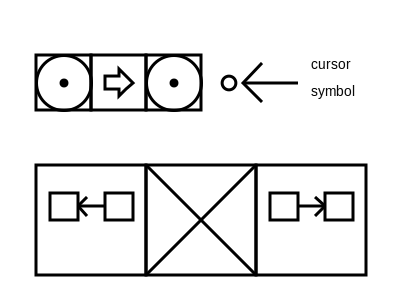
\includegraphics[width=3in]{figures/web2d/cursoredit.png}
	\caption[cursoredit]
	{cursor edits.}
\end{figure}

\begin{figure}
	\centering
	\includegraphics[width=4in]{figures/web2d/keyboard.png}
	\caption[keyboard]
	{keyboard.}
\end{figure}

\begin{figure}
	\centering
	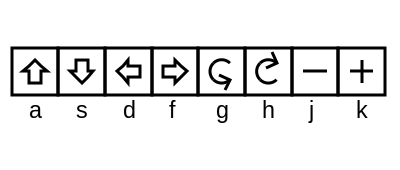
\includegraphics[width=4in]{figures/web2d/move.png}
	\caption[move]
	{Movements.  Arrows move along directions of the lines in the cursor.  Rotation is by the unit indicated by the cursor wing angles. Scale actions are by the current scale value as shown by the dot positions on the cursor.  Letters shown indicate the keys which map to these actions on a QWERTY keyboard with the default settings.}
\end{figure}

\begin{figure}
	\centering
	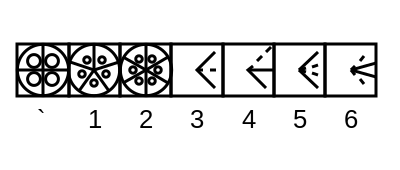
\includegraphics[width=4in]{figures/web2d/angles.png}
	\caption[angles]
	{Angles described by symmetry glyphs.  This also shows the actions to bisect, double, trisect and triple angles, and what keys are used to activate each geometric action.}
\end{figure}

\begin{figure}
	\centering
	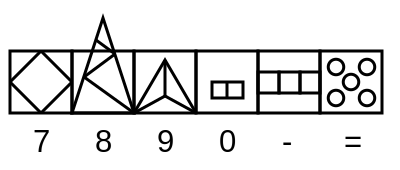
\includegraphics[width=4in]{figures/web2d/scaleactions.png}
	\caption[scaleactions]
	{Scales, along with keys used to map to them in default configuration. There is no relation between the numbers on the keys and the mathematics of the scales.  The scales shown are, from left to right, the square root of 2, the Golden Ratio, the square root of 3, 2, 3, and 5.}
\end{figure}

\begin{figure}
	\centering
	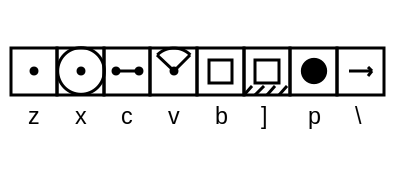
\includegraphics[width=4in]{figures/web2d/basicdraw.png}
	\caption[basicdraw]
	{Basic drawing actions, along with keys used in default configuration to activate them.  From left to right the actions are: draw dot, draw circle of unit radius, draw line segment of unit length, draw arc between cursor wings, draw a square, draw a filled square, draw a filled circle, and draw a line segment while moving forward one unit.}
\end{figure}

\begin{figure}
	\centering
	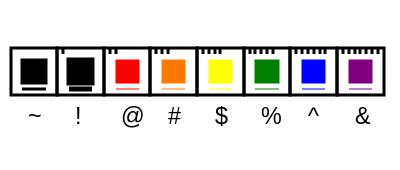
\includegraphics[width=4in]{figures/web2d/colors.png}
	\caption[colors]
	{Layers. Each layer has a line color, line width, and fill color, all of which are set with the Style object using the Style editor app.}
\end{figure}


\begin{figure}
	\centering
	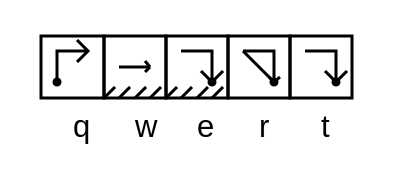
\includegraphics[width=4in]{figures/web2d/pathactions.png}
	\caption[pathactions]
	{Path actions, with keys used to activate them in default state.  From left to right, actions are: start path, draw line segment in path, close a filled path, close an unfilled path, and terminate a path without closing it.}
\end{figure}

\begin{figure}
	\centering
	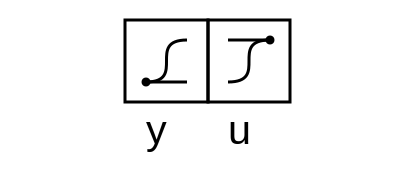
\includegraphics[width=4in]{figures/web2d/bezieractions.png}
	\caption[bezieractions]
	{Start a Bezier Path and terminate it with the y and u keys.}
\end{figure}


\begin{figure}
	\centering
	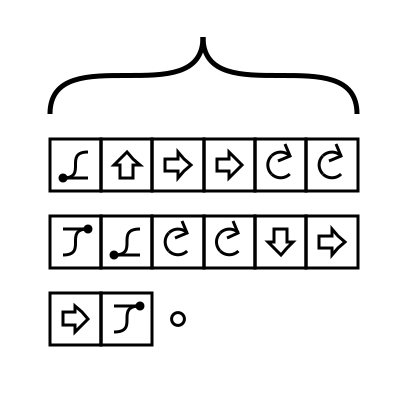
\includegraphics[width=4in]{figures/web2d/bezierbracket.png}
	\caption[bezierbracket]
	{Demonstrating the power of Geometron to make useful symbols with Bezier paths quickly and easily: a twiddle bracket.}
\end{figure}


\begin{figure}
	\centering
	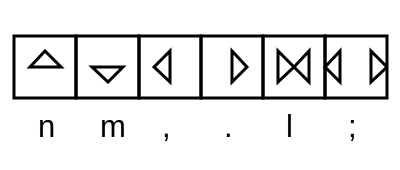
\includegraphics[width=4in]{figures/web2d/panzoom.png}
	\caption[panzoom]
	{Pan and zoom the field of view.}
\end{figure}

\begin{figure}
	\centering
	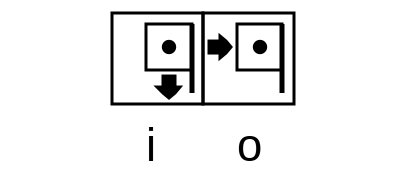
\includegraphics[width=4in]{figures/web2d/flagactions.png}
	\caption[flagactions]
	{Drop a flag, return to flag.}
\end{figure}


\begin{figure}
	\centering
	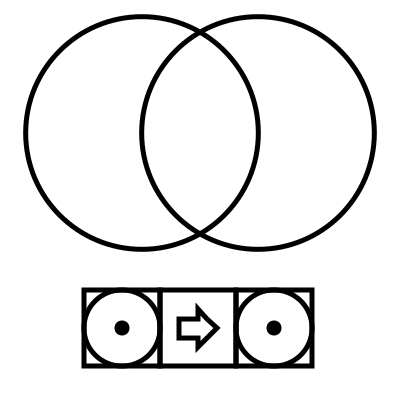
\includegraphics[width=4in]{figures/web2d/vesicapiscis.png}
	\caption[vesicapiscis]
	{The ``hello world'' of geometric programming, the Vesica Piscis.}
\end{figure}
\begin{figure}
	\centering
	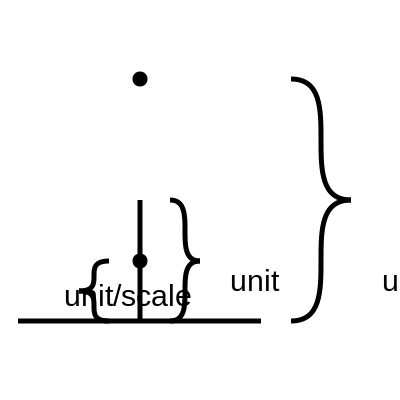
\includegraphics[width=4in]{figures/web2d/cursorscale1.png}
	\caption[cursorscale]
	{Cursor scale.}
\end{figure}
\begin{figure}
	\centering
	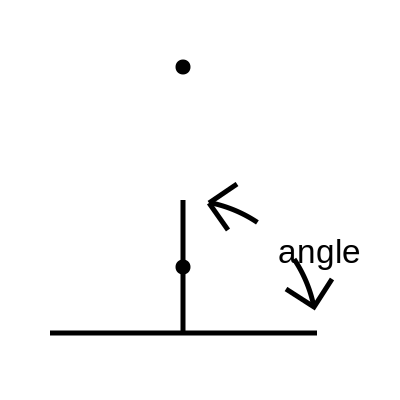
\includegraphics[width=4in]{figures/web2d/cursorangle1.png}
	\caption[cursorangle]
	{Cursor angle.}
\end{figure}
\begin{figure}
	\centering
	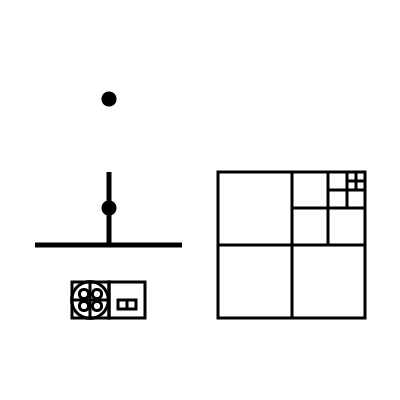
\includegraphics[width=4in]{figures/web2d/cursorsquare.png}
	\caption[cursorsquare]
	{Cursor square.}
\end{figure}
\begin{figure}
	\centering
	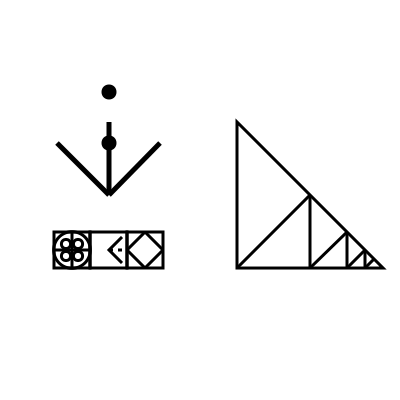
\includegraphics[width=4in]{figures/web2d/cursorroot2.png}
	\caption[cursorroot2]
	{Cursor root2.}
\end{figure}
\begin{figure}
	\centering
	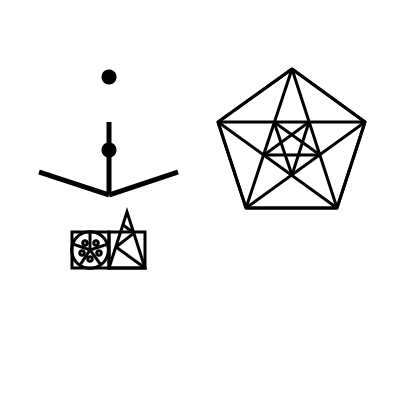
\includegraphics[width=4in]{figures/web2d/cursorgolden.png}
	\caption[cursorgolden]
	{Cursor golden ratio.}
\end{figure}
\begin{figure}
	\centering
	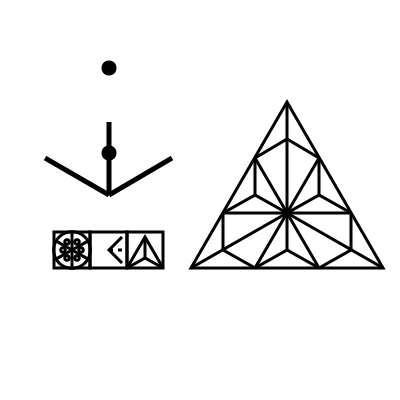
\includegraphics[width=4in]{figures/web2d/cursorroot3.png}
	\caption[cursorroot3]
	{Cursor root 3.}
\end{figure}
\begin{figure}
	\centering
	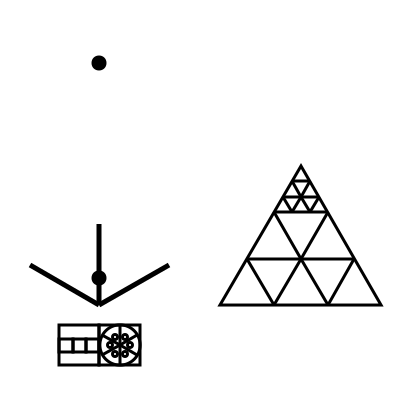
\includegraphics[width=4in]{figures/web2d/cursor3.png}
	\caption[cursor3]
	{Cursor 3.}
\end{figure}
\begin{figure}
	\centering
	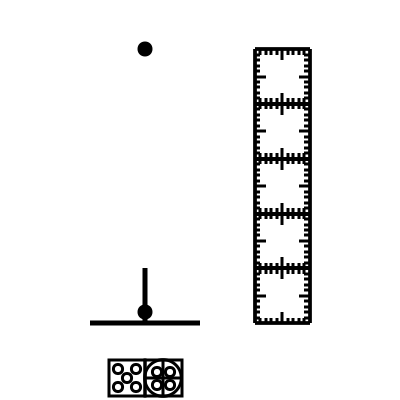
\includegraphics[width=4in]{figures/web2d/cursor5.png}
	\caption[cursor5]
	{Cursor 5.}
\end{figure}


\subsection{Style}

Each instance of the Geometron Virtual Machine has a style object, which defines 8 layers, numbered from 0 to 7.  Each style has a line color, line width, and fill color.  The properties of the style object are stored in the JSON file data/currentjson.txt which is used by the app symbol.html to edit graphics which are used by the rest of the Geometron system.  

\begin{figure}
	\centering
	\includegraphics[width=4in]{figures/web2d/styleeditor.png}
	\caption[styleeditor]
	{Screen shot of the style editor app at styleeditor.html.  The display on the right hand side of the screen shows an unfilled circle and filled circle of each layer's style.  The text area in the bottom left of the screen is used to import and export style data, which can be saved offline and shared with other users via text message, email, etc.  The RESET button resets the style to a standard setting, which will erase any changes made to the existing style. Enter new values into any field to immediately change it.}
\end{figure}

While the style app edits the data file currentjson.txt which applies to the whole Geometron object used for symbol editing, the importing and exporting of data for sharing with other users only includes style information, without the rest of the JSON data.  This allows styles to be separated from the rest of the information for the purposes as usual of building a robust remix culture where Geometron users can constantly be sharing each piece of the system.  The EXPORT button will always post the current style JSON in the window in the lower left of the screen.  IMPORT will import the data, and RESET returns it to a default state.  Try creating your own new style with unusual line widths and colors, then exporting it and saving it offline, sharing it with other users, etc.  

Colors are in the format of HTML/CSS/JavaScript, and can be either names of colors like ``red'' or RGB color values like ``\#00ff00''.  This last format is a number in base 16 which has three 2 digit numbers in it(numbers between 0 and 0xFF), where the three numbers are values of red, green, and then blue.  So black is \#000000 and white is \#FFFFFF.  Any value where all three numbers are the same, like \#808080 will be a shade of grey.   Colors can be partially transparent by adding a fourth hexidecimal number which represents opacity.  So fully opaque red is \#FF0000FF, and red with half transparency is #FF000080(80 because 8 is half of 16, this is actually 128 in decimal).

\subsection{Graphics Setup}

The next section of the JSON we want to know how to edit in order to be able to make useful graphics is the setup, edited in the app setup.html.  Setup edits five numbers, all of which are in units of pixels: x0, y0, unit, width and height.  Width and height are the width and height of the graphics file currently being edited or created.  When a Geometron glyph is drawn with a given GVM, it starts with x and y equal to x0 and y0. Setting these two values is therefore effectively setting the horizontal and vertical offset of the field of view of the symbol.  When we activate a pan function within the symbol.html app what we are really doing is modifying the values of x0 and y0 in the JSON file.  These are done manually in this app.  Finally, unit describes the initial unit value of the GVM.  This is essentially the scale factor.  So again when we activate the zoom functions in any other symbol editor what we are really doing is making changes to the variable unit in the global JSON file.    

The app setup.html has five fields in which to enter the numbers for the five values. There is also a reset button to restore default, with a 600 by 600 pixel square and 80 pixel unit centered in the center.  

\subsection{The Shape Stack}

The final section of the global JSON file which defines the settings of the symbol app is the shape stack.  This is a subset of the hypercube, and is stored both in the JSON file data/hypercube.txt and also data/currentjson.txt.  When vector graphics files are saved, this shape stack is stored inside them so that they can be reloaded with the whole stack.

Exchange of shape stacks. Manual retrieval from .svg files.  uploaded svg files and click to load the whole json.

control panel

hypercube editor for manual direct control

font editor, font.html editing data/hypercube.txt


keyboard editor

symbol trace, saves to symbol feed, which can get loaded, links to globalimagefeed, localimagefeed

work flow with glyph strings, copy paste from all the inputs to all the inputs

\subsection{laser cut designs}

\begin{itemize}
\tightlist
\item
hello world vesica piscis
\item
symbols, how they work with hypercube, 
\item
editing, cursor, keyboards, control panels, modes
\item
symmetries and scales, different methods of geometron(AG)
\item
cursor,movements, basic constructions(segment, circle, arc, dot)
\item
layers, colors, lines, style json, working with styles, transparency in hex colors, finding colors
\item
bezier curves
\item
paths
\item
character stack
\item
fonts
\item
flags
\item
tracing symbols from images
\item
editing the hypercube and shape table, sharing them, import and export of hypercube, sharing of bytecode
\item
canvas,svg/png/base64 workflow, laser cut shapes production, practical graphics for manuscripts and web, iconsymbols, usage in jupyter notebooks, how the JSON embeds in the SVG, how the symbol feed works, how the setup of JSON works,
\item
control panels, softkey interfaces, writing geometron apps, how to replicate in other systems from scratch
\item
examples of using the GVM in JS, documentation of geometron.js, how to use just as a js library to build whatever you want, a list of things someone needs to build to make all this a lot better, how to do that
\end{itemize}
\chapter{Shapes and Fonts}
\section{shapes and fonts: examples}

\begin{figure}
	\centering
	\includegraphics[width=4in]{figures/shapes/rlc.png}
	\caption[RLC]
	{RLC circuit.}
\end{figure}

\begin{figure}
	\centering
	\includegraphics[width=4in]{figures/shapes/rcline.png}
	\caption[RCline]
	{RC line circuit.}
\end{figure}


\begin{figure}
	\centering
	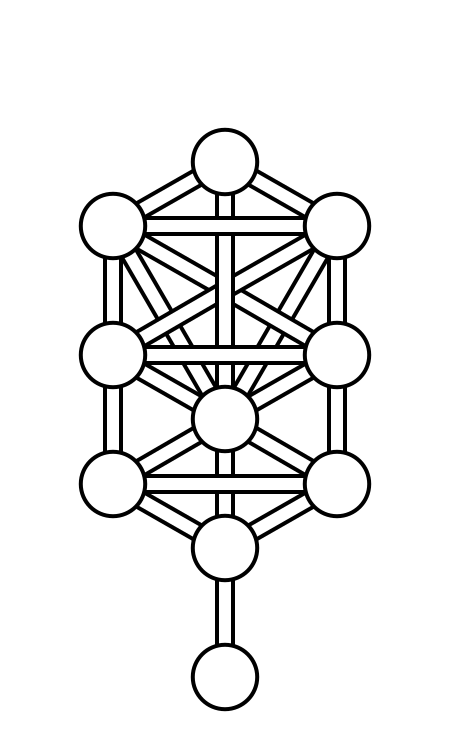
\includegraphics[width=4in]{figures/shapes/treeoflife.png}
	\caption[treeoflife]
	{The Tree of Life from Jewish mysticism.}
\end{figure}

\begin{figure}
	\centering
	\includegraphics[width=4in]{figures/shapes/treeoflifespelling.png}
	\caption[treeoflifespelling]
	{Symbol glyph spelling of Tree of Life. What makes things like this easy to make is building up building blocks like the cross pieces of all different scales, and the use of universal symmetries and scales(6 fold, 12 fold, and the square root of 3 and 2).}
\end{figure}

\begin{figure}
	\centering
	\includegraphics[width=4in]{figures/shapes/estrogendiagram.png}
	\caption[estrogendiagram]
	{Molecular symbol for the steroid hormone estrogen.  Note the characteristic hexagon-pentagon combination which is repeated throughout self-replicating chemical systems(life) as well as throughout the Geometron system/language.}
\end{figure}

\begin{figure}
	\centering
	\includegraphics[width=4in]{figures/shapes/estrogenspelling.png}
	\caption[estrogenspelling]
	{Symbolic spelling of the chemical symbol in the previous figure.  This spelling is only possible because of constructing a symbolic language specific to drawing organic chemistry symbols.}
\end{figure}

describe in detail in this section the work flow for shape stack and fonts, with sharing of fonts, import and export, use of tracer app to trace in fonts and symbols.  Link to scrolls which have code to copy/paste of various fonts.  

This section documents font.html, hypercube.html, shapestack.html, shapestacksymbols.html.  How to use each one, workflow with each.  Examples of each.  

As with Trash Robot, this chapter does NOT need to document each thing, show each font, etc.  This chapter describes the workflow, how to learn, how things work, but then points to a scroll included with each instance of the System which actually has the various examples linked.  This scroll still needs to be written.  All the numerous examples will go in the scroll!  Scroll can have links to pastebins, so that it is minimal in size.



this chapter is only examples. the whole workflow and structure is in the previous chapter, including how to make a font, edit, share, examples of very elementary symbolic languages.  This is just a gallery of examples with links to the actual files for users to copy/paste and use.

\begin{itemize}
\tightlist
\item
editing shape stack, workflow, how to share, upload, download, send and store, same with fonts, connect to hypercube
\item
basic shapes built into 0200 thru 0217, how it's all connected to 01xxx
\item
pixel fonts
\item
laser cut fonts
\item
signal flag font
\item
general circuits
\item
quantum circuits
\item
organic chemistry diagrams
\item
graph theory, with digression into how to operate Maps with mathjax formatting for fully tex compatible graph theory figure creation
\item
quantum logic gates
\item 
classical logic gates
\item
standardized icon design for geometron system
\item
katakana
\item
hebrew
\item
laser cut shape set shape stack
\item
laser cut ruler
\item
laser cut protractor
\item
tree of life from western occult practice
\item
penrose tiles, fun with golden ratio, fivefold symmetry
\item
cross stitch design
\end{itemize}
\chapter{Machine Control}
\section{Machine Control}

\begin{itemize}
\tightlist
\item
introduction, the democratization of automation
\item
structure of hypercube, workflow, general principles
\item
trash robot printer
\item
wall robot on large building
\item
agricultural robot prototype/description
\item
dual winch robot
\item
electron beam lithography
\item
hacked 3d printer to make 2.5d printer
\end{itemize}
\chapter{Geometron in 3d and Beyond}

\section{Geometron in 3d and Beyond}


\subsection{Structure, Definitions and Formats}

\begin{figure}
	\centering
	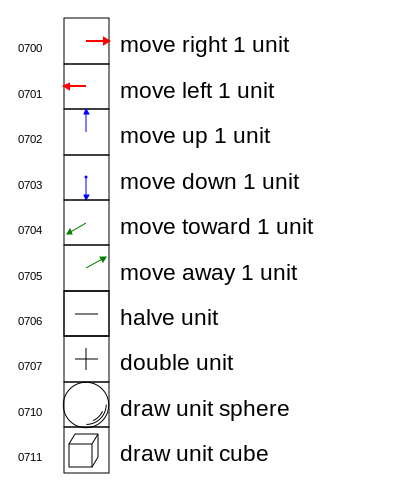
\includegraphics[width=4in]{figures/geometron3d/actions.png}
	\caption[actions3d]
	{Actions.}
\end{figure}

Whimsy Castle

\begin{figure}
	\centering
	\includegraphics[width=4in]{figures/geometron3d/whimsycastle.png}
	\caption[whimsycastle]
	{castle 3d.}
\end{figure}


\begin{figure}
	\centering
	\includegraphics[width=4in]{figures/geometron3d/whimsycastleturret.png}
	\caption[whimsycastleturret]
	{Turret construction.}
\end{figure}

\begin{figure}
	\centering
	\includegraphics[width=4in]{figures/geometron3d/whimsycastlespelling.png}
	\caption[whimsycastlespelling]
	{whimsycastlespelling.}
\end{figure}


\begin{figure}
	\centering
	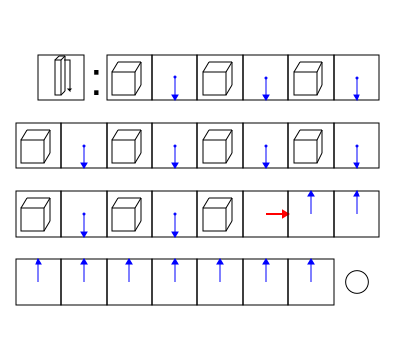
\includegraphics[width=4in]{figures/geometron3d/shapebuilding1.png}
	\caption[shapebuilding1]
	{shapebuilding1.}
\end{figure}

\begin{figure}
	\centering
	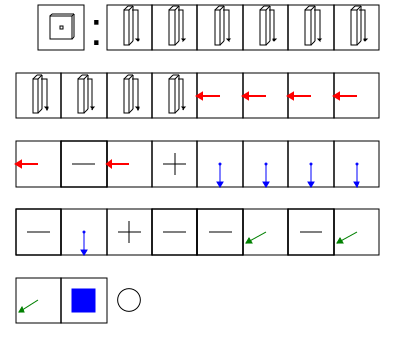
\includegraphics[width=4in]{figures/geometron3d/shapebuilding2.png}
	\caption[shapebuilding2]
	{shapebuilding2.}
\end{figure}

\subsection{Icons and Trash Robot}


\begin{figure}
	\centering
	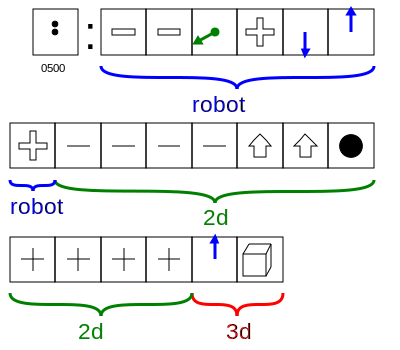
\includegraphics[width=4in]{figures/geometron3d/robot0500.png}
	\caption[robot0500]
	{robot0500.}
\end{figure}

\begin{figure}
	\centering
	\includegraphics[width=4in]{figures/geometron3d/trashrobot3d.png}
	\caption[trashrobot3d]
	{trashrobot3d.}
\end{figure}

\subsection{Rotations and Higher Dimensions}



\begin{figure}
	\centering
	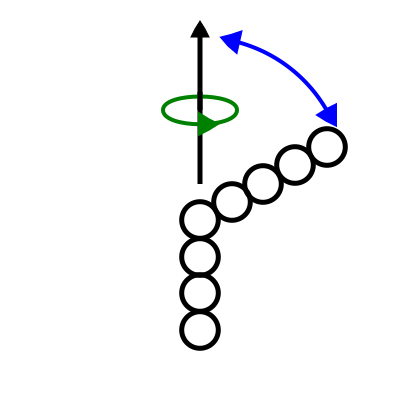
\includegraphics[width=4in]{figures/geometron3d/angles.png}
	\caption[angles]
	{angles.}
\end{figure}

\subsection{Virtual and Augmented Reality, the 3d Web and Games}

\begin{itemize}
\tightlist
\item
  where it exists in hypercube, concepts of movement and construction, cursor
\item
  file formats and software: THREEjs, .x3d, how they are used, 3d printing
\item
  fonts: examples of pixel font of standard English letters and braille with hemispheres
\item
  rotation angles of many part robotic arm tools
\item
  quantum geometron: rotations in hilbert space, representation of hypercube in state of quantum processor, direct mapping to protein folding without gates 
\item
  writing 3d geometron apps, how to use, how to expand and rewrite
\item 
  detailed documentation of the code
\end{itemize}
\chapter{Full Stack Geometron}
\section{Full Stack Geometron}
\begin{itemize}
\tightlist
\item
end goals
\item
hybrid fabrication technology
\item
clockless operation, hardware GVM
\item
image stack, hardware map processing
\item
roctal, storage hardware, scaling, read/write/operate
\item
large projections in Skeletron booths, Geometron station, fully immersive VR/AR at 2 meter scale
\end{itemize}

\subsection{Goals}

Our end goal is an information technology which has zero mined materials.  Every material input in the creation of any technology in our system should come from either a waste stream or from the living world in a closed loop(e.g. naturally harvested sticks and tree sap, goose guano). 

Our initial goal has been to rely on the most open and lowest cost off the shelf hardware possible, which right now is the Raspberry Pi.  As the system expands we will want more and more ways to fully wipe hard drives and sim cards and replace them with Raspberry-Pi-like systems running some form of Linux, with web servers installed with PHP running the same sofwtware. That will be the next step after the Pi phase.  But after that we will try to break up the system into modular parts which can be scavenged from more and more destroyed electronics.  

We see this as a continuous transition where in the beginning we are just running an app on an existing phone, then we wipe the phones and run our own OS, and then we start taking screens, batteries, and other components out and mixing and matching them.  It is in this mixing and matching where the next phase of development will happen.

As this mix-and-match upcycled Linux system evolves, the Trash Robot will also evolve more elaborate ways to fabricate electrical connections at the millimeter scale.  This will eventually lead to more and more complex circuits being built up from scratch, connecting various upcycled components at the individual level(a single resistor, capacitor or MOSFET for instance).  When these circuits can be fully integrated in three dimensions into collections of upcycled components, and when we have some degree of automation in this process, we can start to say we have a fully upcycled system.


The Trash Robot technology can, when it is expanded, be the basis of a milimeter scale interconnect fabrication technology.  Circuits can be immersed in an electrolyte solution and an electrochemical probe controlled with the Trash Robot can 
\chapter{Ontology}
\input{ontology.tex}
\chapter{Trash Robot}
\section{Trash Robot}

Everything here refers back to Ontology.  We build this thing, show how to replicate it, show how replication can benefit the replicator, which stimulates further replication.  Build things and sell them. Build things and use them. Build things and share them for mutual aid and benefit. 

\begin{verbatim}
Trash Robot = {
    ArtBox,
    Trash Tie,
    Tape Snake,
    Token Printer,
    Terminal,
    Brand,
    Textile,
    Shop,
    skeletron,
    constructions
}
\end{verbatim}
    
\begin{verbatim}
constructions = {
    duct tape, 
    cardboard, 
    trash ties, 
    HDPE sheets
}
\end{verbatim}
\begin{verbatim}
shop = {
    ArtBox purse, 
    Trash Robot branded clothes, 
    laser cut acrylic, 
    token printer kits,
    tokens,
    pendants,
    printed bottle caps,
    terminal install
}
\end{verbatim}

\begin{verbatim}
laser cut acrylic = {
    golden triangles, 
    penrose tiles, 
    full set, 
    ruler,
    protractor,
    custom shape,
    spray stencils
}
\end{verbatim}

\begin{verbatim}
printer = {
    brain,
    controller,
    mechanicals,
    workflow
}
\end{verbatim}

\begin{verbatim}
    printer workflow = {
        build, share, sell, use printers, following instructions on scrolls on Geometron
        use Geometron server to follow the rest of this workflow: 
        image feeds,
        aligner,
        trace,
        share feed with other users, save, copy, paste, share share share!!
        load code into Arduino, print in clay tablet, bake it, sell or give away or use
        use print to create stamp, sell or give away or use,
        use stamp to create both coin-like tokens and pendants, stamping in clay, baking, using paint pen and sanding flat, sell, trade, or wear
    }
\end{verbatim}
    

%\printindex

%https://www.sharelatex.com/learn/Glossaries

\end{document}